Below is an overview of the entire system. Data collection from several rooms are performed simultaneously, and processed data is presented to the user through a web page.

\vspace{0.5cm}
\begin{figure}[htb]
	\centering
	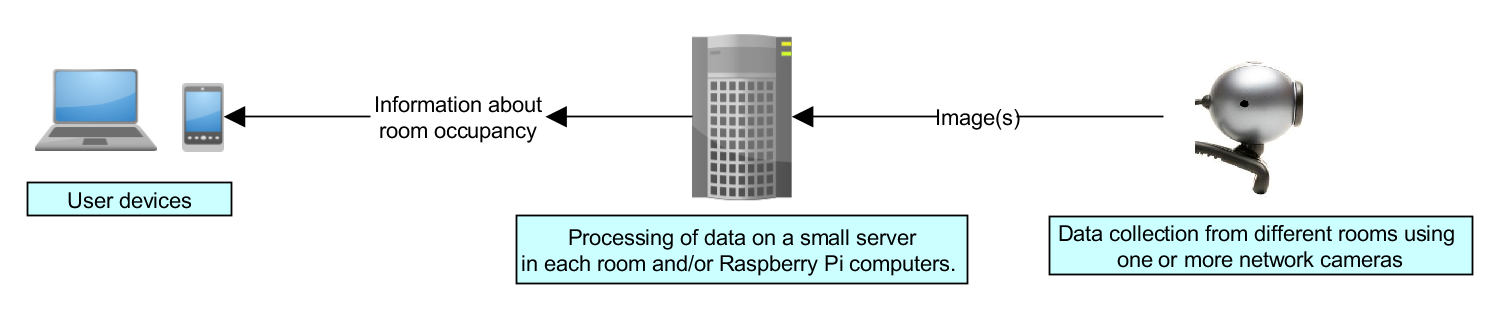
\includegraphics[width=170mm]{images/system_overview.png}
	\caption[System overview]{\textit{A simplified overview of the system}}
	\label{fig:block_overview2_fig}  %Skapar referens till figuren
\end{figure}

\subsection{Rough description of the system}
The camera(s) used to collect data are connected to a local network via Ethernet cables. The main program collects data from the cameras in a room to perform an estimation of room usage intensity, which is then presented to the user in an understandable format, e.g. estimated waiting time.

\subsection{Components}
The main components of the system is of course the cameras, as well as the software running on the central server.

\subsubsection{Hardware}
The cameras are network cameras powered via Ethernet cable, mounted in way that allows for good performance and low installation costs. The hardware is described more thoroughly on this in section \ref{sec:hardware}.

\subsubsection{Software}
The software will be running on a central server, where both image processing and estimation of queue size and waiting time takes place. For a more thorough description of the image processing and estimation programs, see section \ref{sec:software}.

\subsection{Usability and installation}
In order to create a system that is cheap to use and install, it needs to be easy to set up, which is why a user's manual and an installation/calibration program is provided with the system if necessary. As for the usability, relevant data is presented to the user on a web page (see section \ref{sec:usage}). 

